\section[Desenvolvimento do Projeto]{Desenvolvimento do Projeto}

\subsection{Repositório do Código Fonte do Projeto}

O projeto \textbf{VínculoHub Portal} foi organizado em um repositório principal no GitHub, contendo as aplicações de frontend e backend, a documentação técnica, os arquivos de infraestrutura e os scripts de apoio ao desenvolvimento.

\begin{itemize}
    \item Repositório principal: \url{https://github.com/VinculoHub-Portal/VinculoHubPortal}
\end{itemize}

A estrutura do repositório foi dividida principalmente entre as pastas \texttt{frontend}, \texttt{backend} e \texttt{docs}. A pasta \texttt{frontend} concentrou a aplicação web utilizada pelos diferentes perfis de usuário. A pasta \texttt{backend} reuniu a API, as regras de negócio, a integração com banco de dados, autenticação, documentos e serviços externos. A pasta \texttt{docs} foi utilizada para registrar materiais de apoio, validações de sprint, tarefas refinadas e a modelagem do banco de dados.

Além disso, o projeto possui arquivos de orquestração e infraestrutura, como \texttt{docker-compose.yml}, \texttt{docker-compose.dev.yml}, \texttt{docker-compose.swarm.yml} e \texttt{main.tf}, evidenciando uma preocupação com padronização de ambiente, execução local e preparação para deploy em nuvem.

\subsection{Banco de Dados Utilizado}

O banco de dados utilizado no projeto foi o \textbf{PostgreSQL}. A aplicação também utilizou \textbf{Flyway} para versionamento e execução das migrações do banco, permitindo que a estrutura fosse reproduzida de forma consistente nos ambientes de desenvolvimento e deploy.

A modelagem do banco foi documentada em formato DBML no arquivo \texttt{docs/db/vinculo\_hub.dbml}. Entre as principais entidades modeladas estão usuários, ONGs, empresas, projetos, documentos, editais, ODS, endereços, denúncias e vínculos entre empresas e projetos.

\begin{figure}[H]
    \centering
    \small
    \caption{Modelagem do banco de dados do VínculoHub Portal}
    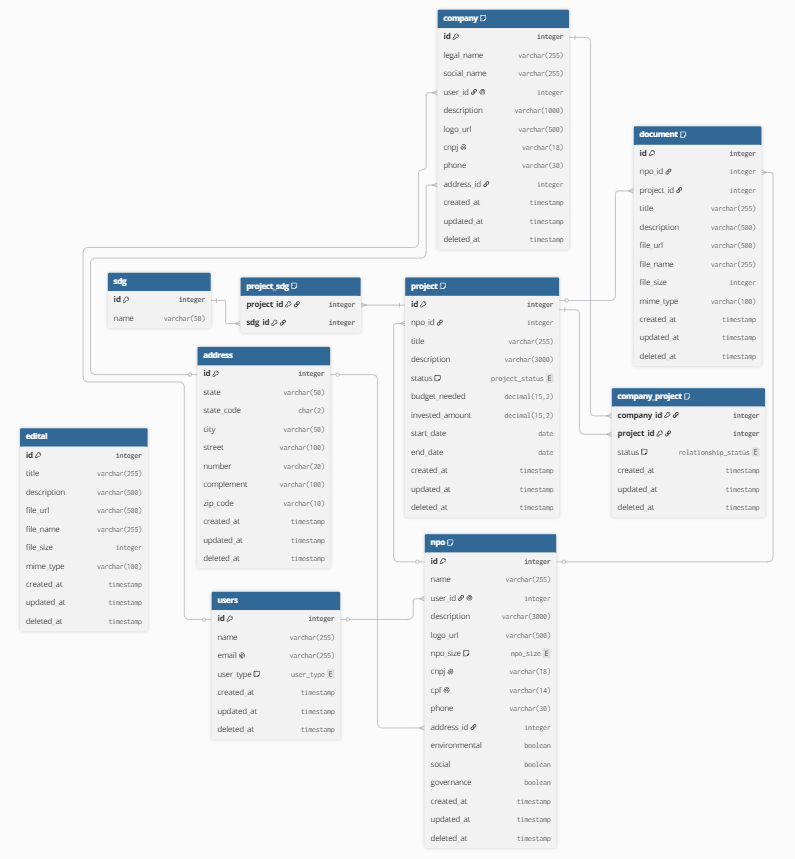
\includegraphics[width=1\linewidth]{conteudo/4 - ages III/conteudo/figures/banco-dados-vinculohub.png}
    Fonte: Documentação do projeto VínculoHub Portal
    \label{fig:vinculohub-banco-dados}
\end{figure}

A entidade \texttt{users} armazena os dados básicos do usuário e mantém integração com o Auth0 por meio do campo \texttt{auth0\_id}. As entidades \texttt{npo} e \texttt{company} representam, respectivamente, ONGs e empresas cadastradas na plataforma. A entidade \texttt{project} centraliza os projetos cadastrados pelas ONGs, enquanto \texttt{document} armazena metadados de arquivos vinculados a ONGs ou projetos. A tabela \texttt{company\_project} representa os vínculos entre empresas e projetos, com status como pendente, em negociação, ativo ou inativo.

\subsection{Arquitetura Utilizada}

A arquitetura do projeto foi baseada em uma aplicação web separada em frontend, backend, banco de dados e serviços externos. O frontend se comunica com o backend por meio de API REST. O backend centraliza as regras de negócio, validações, persistência dos dados, segurança e integrações externas. O banco PostgreSQL armazena os dados relacionais da aplicação.

A autenticação e autorização foram integradas ao \textbf{Auth0}, com separação de perfis por roles, como \texttt{COMPANY}, \texttt{NPO} e \texttt{ADMIN}. Essa separação permitiu controlar o acesso às rotas e funcionalidades específicas de empresas, ONGs e administradores.

O projeto também utilizou \textbf{Docker Compose} para execução local dos serviços, incluindo backend, frontend, banco PostgreSQL e Flyway. Para armazenamento de arquivos, como documentos e editais, foi prevista integração com \textbf{AWS S3}. A documentação e os arquivos de infraestrutura também indicam uma organização voltada a deploy em ambiente AWS, com uso de EC2, Docker Swarm, Elastic Block Storage e bucket S3.

\begin{figure}[H]
    \centering
    \small
    \caption{Arquitetura de infraestrutura do VínculoHub Portal}
    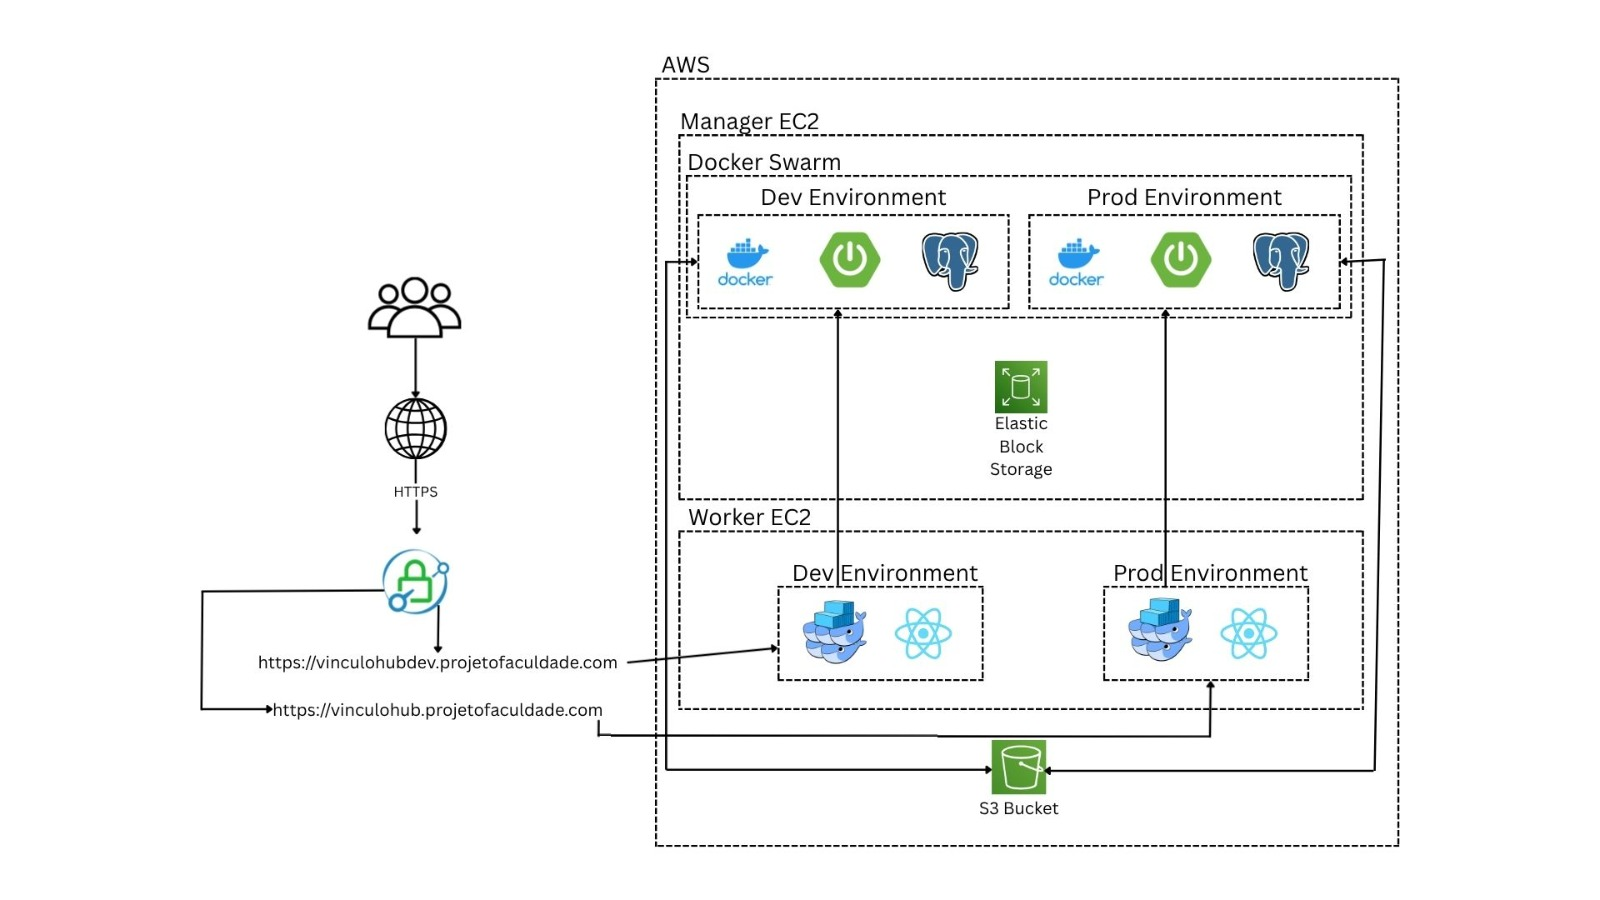
\includegraphics[width=1\linewidth]{conteudo/4 - ages III/conteudo/figures/arquitetura-vinculohub.jpeg}
    Fonte: Documentação do projeto VínculoHub Portal
    \label{fig:vinculohub-arquitetura}
\end{figure}

Essa arquitetura permitiu organizar ambientes de desenvolvimento e produção, padronizar a execução dos serviços e separar responsabilidades entre interface, API, banco de dados, autenticação e armazenamento de arquivos.

\subsection{Protótipos das Telas Desenvolvidas}

Durante o desenvolvimento do VínculoHub Portal, os protótipos e fluxos de tela serviram como base para a construção das principais experiências da aplicação. Entre os fluxos contemplados estavam o cadastro de ONGs, cadastro de empresas, dashboards por perfil, mural de editais, perfil público de ONGs, perfil público de empresas, cadastro e edição de projetos, upload de documentos, denúncias e gestão de vínculos.

No frontend, esses fluxos foram implementados em páginas e componentes específicos, como \texttt{AdminDashboard}, \texttt{CompanyDashboard}, \texttt{OngProfilePage}, \texttt{OngPublicProfilePage}, \texttt{ProjectDetailsPage}, \texttt{EditaisMuralPage}, \texttt{MyRelationshipsPage} e páginas administrativas para ONGs, vínculos e notificações.

\subsection{Tecnologias Utilizadas}

No frontend, o projeto utilizou \textbf{React}, \textbf{TypeScript} e \textbf{Vite} como base da aplicação web. Também foram utilizadas bibliotecas como \textbf{Material UI}, \textbf{Tailwind CSS}, \textbf{React Router}, \textbf{React Query}, \textbf{Axios} e \textbf{Auth0 React SDK}. Para testes e qualidade do frontend, foram utilizados \textbf{Vitest}, \textbf{Testing Library} e \textbf{Playwright}.

No backend, a aplicação foi construída com \textbf{Java 17} e \textbf{Spring Boot}. A stack incluiu Spring Web, Spring Data JPA, Spring Security, OAuth2 Resource Server, validação, PostgreSQL, Flyway, Swagger/OpenAPI, AWS SDK para S3, Lombok, JUnit, Testcontainers e JaCoCo.

A infraestrutura local foi padronizada com \textbf{Docker} e \textbf{Docker Compose}, permitindo subir frontend, backend, banco de dados e migrações com menor esforço de configuração. Também foram utilizados hooks de Git, Spotless, PMD e SpotBugs como mecanismos de apoio à padronização e qualidade do código.

Entre as funcionalidades técnicas mais relevantes da stack estão: autenticação com Auth0, autorização por roles, upload de arquivos para S3, migrações versionadas com Flyway, documentação de API com Swagger, testes automatizados, cenários E2E com Playwright e endpoints REST para dashboards, projetos, editais, documentos, denúncias e vínculos.
